% experimentacion
\vspace{1em}
Para revisar de manera empírica la cota lineal del algoritmo\footnote{Los experimentos y archivos resultantes se pueden encontrar en \textit{./ej-3/experimentacion}.}, procedimos a implementarlo en $C++$ y realizamos una serie de evaluaciones respecto a su tiempo de ejecución en función del tamaño $n$ de la entrada, para muestras aleatorias con $n = 2^k$ para $k$ natural en el rango $[16,\ 26]$. Realizamos cada evaluación diez veces para reducir la variación de los resultados y tomamos el promedio aritmético. 

El siguiente gráfico describe, en escala \textit{log-log} ---dada la naturaleza exponencial de los casos de test--- la relación entre el tamaño de entrada y el tiempo de ejecución. También, muestra la línea que mejor describe los datos, resultante de aplicar regresión lineal.  
%Luego graficamos el tiempo de ejecución de en función de estos tamaños de entrada, aplicando el logaritmo en ambas entradas para mejorar la visibilidad, dada la naturaleza exponencial de las muestras. Tras aplicar regresión lineal, el gráfico quedó de la siguiente forma:
\begin{figure}[!htbp]
    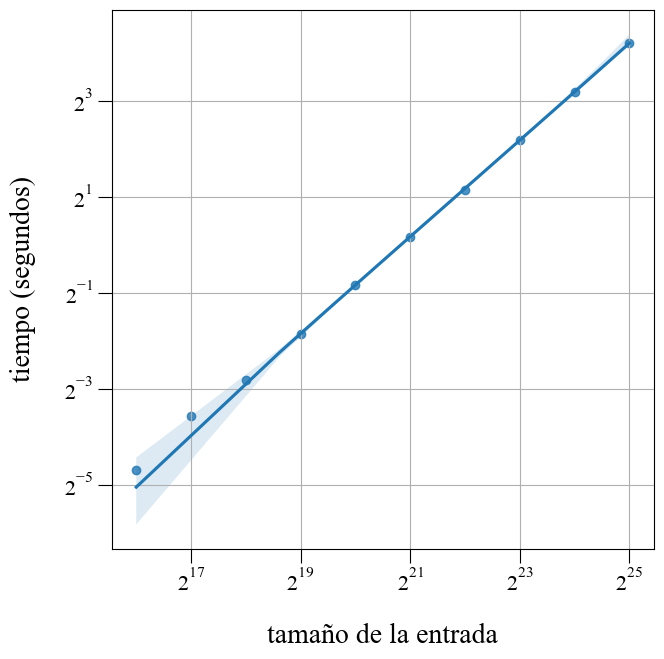
\includegraphics[scale=0.5, clip]{./files/src/.media/aleatorio.png}
    \caption{Tiempo de ejecución del algoritmo de \textit{selección de actividades} en función del tamaño de la entrada, para instancias aleatorias.} \label{aleatorio}
\end{figure}

La relación lineal es bastante clara. Para asegurarnos, calculamos también el coeficiente de Pearson, $\rho$, que mide la correlación lineal entre ambas variables, donde $\rho = 1$ indica una correlación fuerte. El resultado fue $\rho \approx 0.9997$.

% instancias
\subsection{Instancias de interés}

Un análisis rápido del algoritmo indica que lo único que parece alterar el flujo del código, en función de la entrada, es 
la cantidad de actividades que son seleccionadas. Donde, por cada actividad seleccionada, se ejecutan dos lineas de código más (en particular, se agrega un elemento más al conjunto de soluciones $P$). %Sin embargo, de implementarse como proponemos, solo agrega un tiempo de ejecución constante, por lo que no debería ser demasiado significativo.
%cada tupla ordenada empieza después (o al mismo tiempo) que cuando termina la última tarea de P. 

Para probar la diferencia de tiempos posibles entre instancias diferentes bajo este criterio ---que tengan cantidades distintas de actividades seleccionables---, realizamos una serie de evaluaciones, siguiendo la metodología de la experimentación anterior, primero con una instancia \textit{comprimida} ---en la que la intersección entre todos los intervalos de las actividades de $A$ es no vacía, por lo que sólo se agrega un elemento al conjunto de soluciones $P$--- y una instancia de entradas \textit{separadas} ---donde la $i$-ésima entrada tiene la forma $(i,\ i+1)$, por lo que se agregan todas las actividades en $A$ al conjunto de soluciones $P$---. 

El siguiente gráfico, nuevamente en escala \textit{log-log} por la naturaleza de las muestra, expone los resultados.

\begin{figure}[!htbp]
    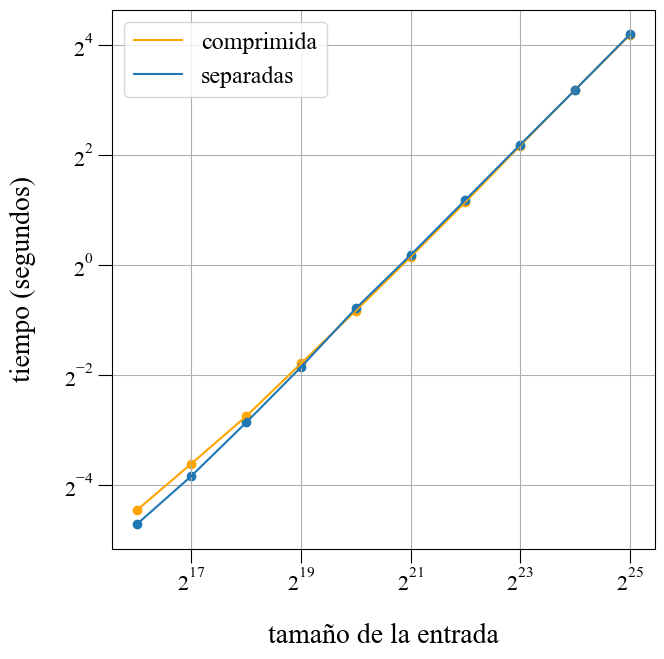
\includegraphics[scale=0.5, clip]{./files/src/.media/comparacion.png}
    \caption{Tiempo de ejecución de \textit{actividades} en función del tamaño de entrada $n$ y la cantidad máxima $m$ de tareas seleccionables, para \textit{comprimida} ---$m = 1$--- y \textit{separadas} ---$m = n$---.} \label{comparacion}
\end{figure}


Si bien es verdad que, en las entradas más grandes, las entradas \textit{separdas} parecen haber tomado un poco más de tiempo, no resulta una diferencia significativa. En promedio, la diferencia entre ambos tipos de entrada fue del $\approx 0.0208$ a favor de \textit{separadas}.